\documentclass[conference]{IEEEtran}
\IEEEoverridecommandlockouts
% The preceding line is only needed to identify funding in the first footnote.
% If that is unneeded, please comment it out.
\usepackage{silence}
\usepackage{cite}
\usepackage{amsmath,amssymb,amsfonts}
\usepackage{algorithm,algorithmic}
\usepackage{graphicx}
\usepackage{booktabs}
\usepackage{textcomp}
\usepackage{mathptmx}
\usepackage{enumitem}
\usepackage{titlesec}
\usepackage{capt-of}

\setcounter{secnumdepth}{4}

\def\BibTeX{{\rm B\kern-.05em{\sc i\kern-.025em b}\kern-.08em
    T\kern-.1667em\lower.7ex\hbox{E}\kern-.125emX}}
\begin{document}

\WarningsOff*

\title{Final Report\\
Blue-Collar Node : A Sharding Approach for Optimizing Storage on Blockchains
}

\author{\IEEEauthorblockN{1\textsuperscript{st} Chawla}
\IEEEauthorblockA{\textit{Computer Science} \\
\textit{Arizona State University}\\
nchawla3@asu.edu}
\and
\IEEEauthorblockN{2\textsuperscript{nd} Saikia}
\IEEEauthorblockA{\textit{Computer Engineering} \\
\textit{Arizona State University}\\
csaikia@asu.edu}
}

\maketitle

\begin{abstract}
    The scalability of blockchain is a primary and urgent concern. The current
    popular blockchains have fundamental bottlenecks which limit their ability
    to have a higher throughput and a lower latency. One of the bottlenecks is
    the storage requirements of the current blockchains. All the full nodes and
    miners in a blockchain are required to store the complete blockchains and it
    grows every time more transactions are added. The network relies mainly on
    commodity hardware for block propagation and transaction verification.
    With the increase in the size of blockchains, storing the entire blockchain
    on voluntary full nodes becomes impractical. Our project focuses at sharding
    this blockchain and storing it in several nodes. There is a two-fold advantage of this,
    transactions can be verified in parallel by different nodes and consensus
    can be achieved in a faster way increasing the throughput of the network,
    and the storage requirement of the full node will be decreased
    substantially. That directly will prevent the blockchain from getting
    centralized towards supercomputers. However, in this project we will focus
    only on the storage part of the problem. Executing transaction in parallel
    will be a part of the future work.
\end{abstract}

\begin{IEEEkeywords}
    blockchain, storage, sharding, blue-collar, decentralized
\end{IEEEkeywords}

\section{Introduction}
In 2009, Bitcoin\cite{bitcoin} introduced the first blockchain which is an
append only database that stores transactions. Blockchain maintains the
distributed database in a decentralized network aiming to solve the Byzantine
Generals Problem \cite{bgp}. Byzantine Generals Problem when extrapolated to
the banking system i.e to digital money translates to double spending problem,
where since there is no material money a malicious node can spend the money
twice, and since there is no central leader to check the money can be
spent.Bitcoin solves this problem by distributing the ledger to
every node in the network and cryptographically securing it making it immutable.
Special nodes called miners try to include the transactions into blocks by
solving a puzzle. This mechanism is called Proof of Work. Each miner then tries
to add this block to the distributed replicated ledger and after the block is
added each node on the network updates their ledger. \\

\subsection{Problems}
Satoshi Nakamoto decided a block interval of 10 minutes between adding 2 blocks
to the chain. The block size was limited to 1MB from "unlimited number of
transaction" because of a DoS attack that happened in 2010.  Since, the block
size is capped and the time interval is constant, the number of transactions
that can be dealt with are limited to ~3-7 transactions per second.  Also, since
the ledger is duplicated on each node on the network, as the ledger grows the
storage requirement of the node increases. 

\section{Background And Related Work}
\\
\subsection{Background}
    Blockchain is a decentralized, tamper-proof digital ledger technology that
    is transforming transaction prospects for many industries. In addition to
    being the foundation of cryptocurrencies like Bitcoin,Ethereum,Dash,etc the blockchain
    structure, which consists of linked blocks of information, allows for direct
    transactions across a network of computers without need for a central
    authority. The Dash network consists of four kind of nodes:
    \textbf{Masternodes}, \textbf{full nodes}, \textbf{light-weight nodes } and \textbf{miners}. Nodes
    save the complete blockchain and have two main functions: 
    \begin{enumerate}[label=(\alph*)]
        \item to validate transactions
        \item to propagate transactions and blocks in the network
    \end{enumerate} 
    Although full nodes validate transactions by checking their inputs and
    outputs, light clients verify transactions by SPV, or by requesting random
    chunks of a block and using the merkle root to verify each chunk. This
    verification technique relies on trust on a full node or the node sending
    data. This can be dangerous, because a malicious node can withhold small
    amount of data and can get unnoticed by many light clients. The network
    becomes much more trustworthy if the number of full nodes are a majority
    since data is always verified. As the blockchain technology is being adopted
    more, the storage requirement is increasing for each individual node. This
    increase in infrastructure requirement forces volunteer nodes to move to
    light-clients. This harms the network in 2 ways :
    \begin{enumerate}[label=(\alph*)]
        \item The network gets more centralized to people who can afford
            supercomputers
        \item The trust on the network weakens as most transactions are not
            completely validated by full nodes
    \end{enumerate}
    In this project, we want to introduce a new kind of node that saves only a
    part of the blockchain thus reducing the storage requirement and also
    validates each transaction that is a part of the block. This will introduce
    the following advantages to the network:
    \begin{enumerate}[label=(\alph*)]
        \item The trust on the network will be high as the nodes will validate
            each transaction fully.
        \item Randomizing block storage in such a way that transactions are
            fully validated by a small part of the network leading to multiple
            transactions being validated in parallel.
    \end{enumerate}
    We will be focusing only on the first advantage as a part of this project,
    the second would remain a future work. \\

\subsection{Related Work}


Elastico \cite{elastico} also attempted sharding by adding the concept of
committees. The complete protocol was revamped by dividing it into 2 rounds. The
first round involves proof of work to choose committees for each node in every
block mining cycle. Once the committees are assigned, nodes use Practical
Byzantine Fault Tolerance \cite{pbft} in order to form a block based on the
transactions that they are to verify. Once transactions are verified, the partial
block is pushed forward to a final committee which finalizes and mines the new
complete block. The throughput of elastic \cite{elastico} increases linearly with
number of committees in the network. This can be shown in the \ref{image: fig2}.

"Sharding FAQ \cite{sharding} gives a good glimpse of the problem we are trying to
solve with techniques that will come in handy for us to make our solution
better.The difference in the approach is that \cite{sharding} tries to scale the
throughput of the blockchain while we focus on the storage optimization of the
system. 

"A note on data availability and erasure coding" \cite{erasureV} is another blog by
the founder of Ethereum \cite{ethY}\cite{ethW} which touches our areas of concerns. It talks
about light clients and how their lack of validation techniques might be harmful
for the network. It exposes a loop-hole in the system which we want to remediate
by the creation of "blue-collar" nodes.

\begin{figure}
    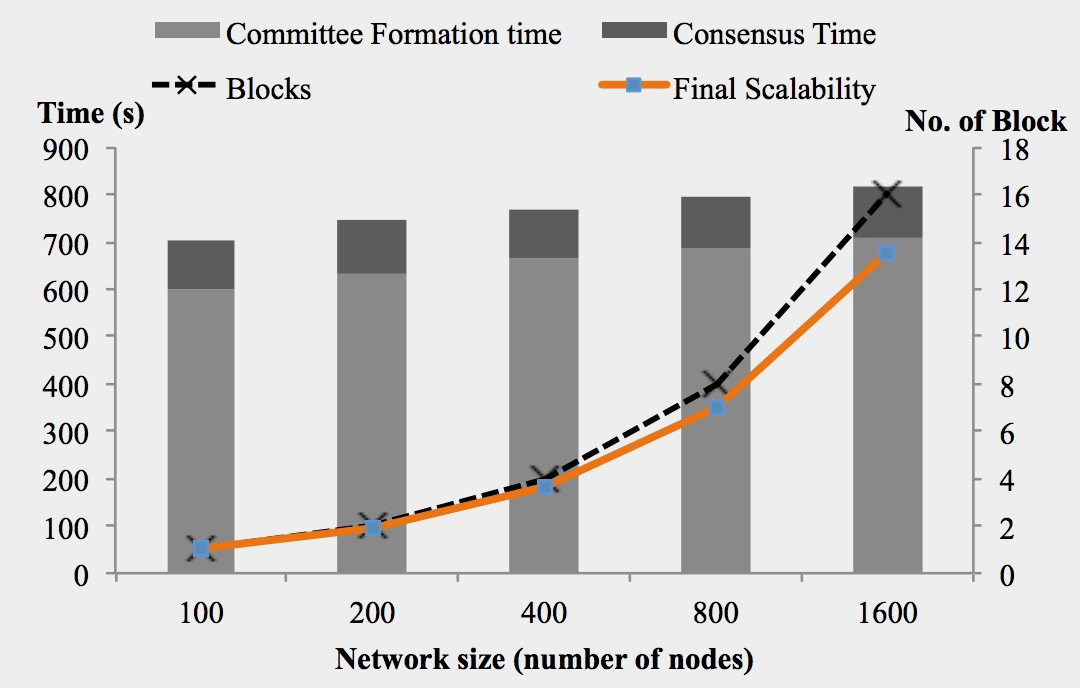
\includegraphics[width=.8\columnwidth]{files/elasticoRes.png}
    \centering
    \caption{Elastico Sharding }
    \label{image: fig2}
\end{figure}
 
\section{Solution: Work In Progress}
\\
\subsection{Components}
The key component of our system will be what we are calling a
\textbf{"Blue-collar node"}.
This node will be a combination of a light and full-node. This node will be
required to store the sharded blockchain and the parity bits such that if needed
it can re-create the data from a connected full node. Creation of shards is done by Erasure Code \cite{erasure}
and currently Reed-Somon algorithm \cite{reed}.

Masternodes are special nodes present in the dash network that have special characteristics.
These are proof of service nodes that are paid a mining awards in order to provide the service.
These masternodes add reliability to the network and can be trusted upon to store the entire blockchain.
Masternodes have high number of connections because they are required to run at 1GBps bandwidth and
most nodes are connected to at least one Masternode.
We will be utilizing this property of masternodes to recreate the data in the newly formed
"Blue-Collar node" that when needs to find a missing transaction pings a Masternode.

However, for open blockchains Kademlia DHT will be used with it's property of 
XOR to find the closest neighbour that has the data.

\subsection{Architecture}
Dash\cite{dash} has a unique privacy-centric infrastructure in place. It employs
4 kind of nodes:
\begin{enumerate}[label=(\alph*)]
    \item \textbf{Masternode}: These are special nodes in the dash network that
        require 1000 dash to be active on the network. These nodes add special
        features to the network such as \textbf{voting} for the proposals that
        are active on the network, \textbf{high-bandwidth} for better relay,
        \textbf{better hardware} for faster transaction processing, etc
    \item \textbf{Full-nodes} These nodes are same as master nodes but are
        voluntary nodes and are a part of network without the need of having a
        1000 dash in their wallets.
    \item \textbf{SPV/Mobile Clients} These are basically mobile clients that
        don't download the blockchain but verify transactions by just combining
        the hashes of merkle tree.
    \item \textbf{Miners} These are nodes that help adding new blocks to the
        blockchain. They require to have a compute intensive hardware in order
        to find the next random number(nonce) that satisfies the difficulty of
        the network.
\end{enumerate}

All nodes apart from the SPV wallets are required to store the entire blockchain
along with indexed leveldb/berkeley db databases in order to verify the
transactions.  \\

\subsection{Challenges}
In the methodology described above there are certain challenges that are not yet
handled. Some of them are listed below:

\begin{enumerate}
    \item The data distribution has to be randomized in such a way that a
        malicious intentions can't get hold of data that can be completely lost.
        In such a case, the contingency would be to recover the data from a full
        node and distribute it again over the network among peers but would
        require a lot of data movement.
    \item The data has to be distributed in such a way that in case some nodes
        fail, the re-distribution of data does not cause much data movement and
        doesn't occupy bandwidth that could be used for block propagation.
\end{enumerate}
\\

\subsection{Theory}
\subsubsection{Erasure Code}
In distributed storage systems, failures are inevitable. Therefore, it is very
important to design these systems with some high availability technique. One way
to do it is by introducing redundancy. One of the well known techniques for
protecting data is erasure coding. It is a widely used and accepted technology
used in communication systems and more recently, in storage systems. In storage
systems, erasure codes add redundancy to the system in order to tolerate
failures. Erasure codes vary from simple coding techniques, such as a full
replication of the data, such as RAID-1, where each byte of the data is stored
on two disks. However, this increases the storage cost. More complex erasure
codes, such as Reed-Solomon codes, exhibit fault tolerance with less extra
storage compared to RAID. Thus, this is a more cost effective approach.

Let's assume that our storage system consists of n disks. These disks can
be partitioned into k disks so that these disks can hold the user data. Thus
the remaining m=n-k disks hold the coding data. The encoding and decoding
techniques are explained in Figure \ref{image: fig3}.

In the encoding process, the contents of the k data disks are used to
calculate the contents of the m coding disks. Thus, this kind of storage
system can handle failure of up to m disks. When any number (up to m) disks
fail, then all the data is decoded from the up and running disks. The
simplest erasure codes assume that each disk consists of one w-bit word.
Optimal erasure codes are maximum distance separable codes. Optimal codes are
expensive in terms of memory usage and CPU time for large value of n. 
The kind of erasure coding used in this experiment are Reed-Solomon codes.
Reed-Solomon codes are MDS codes. For disks where $n<= (2^w)$, Reed-Solomon
codes are usually used. For example, for storage systems which contain
less than or equal to 256 disks, Reed-Solomon is defined for it.
Reed-Solomon codes operate on a block of data treated as a set of finite
field elements called symbols. For example, a block of 4096 bytes can be
considered as a set of 2731 12 bit symbols. Here, each symbol is a finite
field element of $GF(2^12)$ and the last symbol is padded with four 0 bits.
There are different ways to define the $a_ij$ coefficients and one of
them is the "Cauchy" construction. A distinct number n is chosen in $GF(2^w)$ and
then the disks are partitioned into two sets X and Y. X set has m elements
and Y has k elements. Then, 

$a_ij = 1/(x_i \oplus y_i),$
where the arithmetic is over $GF(2^w)$.

Any value of k and m generates result. However, they are expensive since
complexity of multiplication in a Galois Field \cite{gfcomplete} is more expensive then XOR. 

\begin{figure}
    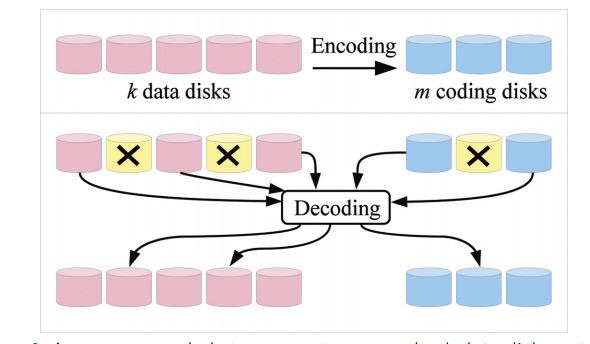
\includegraphics[width=.8\columnwidth]{files/erasure.png}
    \centering
    \caption{Erasure Encoding and Decoding }
    \label{image: fig3}
\end{figure}

\subsubsection{Raptor Code \cite{raptor} : Future Work}
Raptor code are rateless erasure code as opposed to Erasure code whose rate is determined by
values \textit{k} and \textit{n} described above. The rateless here means that limitless sequence of encoding
symbols can be generated from source symbols and can be recovered by any subset (k symbols) of 
encoding symbols that are only slightly larger than the original symbols. These have linear encoding and decoding time
as opposed to Erasure code that exhibit a quadratic time. 
Since these codes are faster in decoding, it has a potential use case of decoding large files that are continuously
broadcasted to a set of receivers.
Raptor codes are heavily covered in patents as of now, therefore currently Erasure codes have been used for this project.



\subsubsection{Distributed Hash Table: Kademlia : Work In Progress }
We are in the process of using openDHT \cite{opendht}, which is an open source library
developed by UC Berkeley for implementing Distributed Hash Tables. We have chosen Kademlia over other
hash table structures like chord because Kademlia contacts only $O(log n)$ nodes in order
to retrieve the location of the information.

Since we are able to implement erasure codes, DHT will help us dissipate that information, update the table.
The decoding function is already written. It is not yet integrated with the original code, because in order to
decode we would require the location of the data.


\subsection{Implementation}

The implementation is done in 3 parts: \\

\subsubsection{The emulator}
Since this is a complex problem to be solved on a decentralized distributed
system. In order to achieve and test the desired results, an emulator was set up
that automates the following process: \\

\begin{enumerate}[label=(\alph*)]
    \item Building dependencies on each node.
    \item Building dash static binaries to form light clients.
    \item Building docker clients with running docker clients.
    \item Forming a network of nodes with random number of connections with
        minimum and maximum set.
\end{enumerate}
\\
\subsubsection{Automating Dash build with Docker}
In this phase we have set up a docker container with all packages statically
built in order to optimize space storage inside the container. We have
used "Ubuntu" as the base image for docker. The dash build is not one of the
release versions but is taken from the "development" branch in order for us to
contribute directly. A combination of shell, python and docker is used to
automate the installation of dependencies along with the original dash client. \\

\subsubsection{Setting up Regression Test Network}
In this phase we have used the same automation tool and cloned many docker
clients with different ports. The dash clients in \textbf{\textit{-regtest}}
mode do not automatically discover new nodes even with
\textbf{\textit{-discovery=1}} flag because the \textit{peers.dat} file that has
a regular feed of peers does not have any seed from the current local network.
In order to rebut that we randomly assigned peers to each node by using the
algorithm Algorithm 1: 

\begin{algorithm}
    \caption{Connect Nodes}
	\begin{algorithmic}[1]
            \WHILE {\textit{numberOfConnections for \textbf{i}} $<$
            \textit{minConnections[i]}  and \textit{count} $<$ 
            \textit{10*minConnections[i]}}
            \STATE {  \textit{index} \gets \text{random(0,numOfNodes*100)} $\%$ \\  \text{(numOfNodes - 1);}  } \\
            \STATE { \textit{candidaePeer} \gets \text{index;}  } \\
            \IF{$ \textit{candidaePeer} == \text{i} $}
            \STATE {\text{\textbf{print} "Can't connect to itself"}}
            \ELSIF { \textit{nodesConnections[i]}  $>=$ \\ \text{maxConnections[candidatePeer]} }
            \STATE {\text{\textbf{print} "Node already has maximum connections" }    }
            \ELSIF {\textit{candidatePeer} in \text{nodesConnections[i]} }
            \STATE { \text{\textbf{print} "Node already has maximum connections" } }
            \ELSE
            \STATE { \text{append} \textit{candidatePeer} \text{to} \textit{nodesConnections[i]}  } }
            \STATE { \text{append} \textit{i} \text{to} \textit{candidatePeer}}
            \STATE { \text{add peer} \textit{candidatePeer} \text{to} \textit{i} }
            \ENDIF
            \ENDWHILE
        \end{algorithmic}
\end{algorithm}
\\

\subsubsection{Adding sharding techniques to the dash original repository and
integrating it our docker-dash network} \\

In order to create erasure codes we are using the write-to-disk methodology in
the original dash code. 
The library Jerasure \cite{jerasure} has been used in order to create erasure codes through
different encoding algorithms with different values of \textbf{\textit{k}} and
\textbf{\textit{m}} in order to find an optimal way of distributing data among
the nodes.

Also, we have changed the parameter \textbf{\textit{MAX\_BLOCK\_FILE}} to 256K
instead of 128 MiB for the ease of testing.

We choose the latest file that has been recently created and is full. We divide that
information into $k+ m$ files. These \textit{m} files are the ones that we can 
lose and still be able to regenerate the data. In addition to these files, a small 4K
meta file is created that consists the encoding parameters.

This meta files must be present on all the nodes that are using the sharded blockchain
in order to recreate the data when needed for verification.


\section{Results}
The following accomplishments have been made during the course of this project:



\begin{tabular}{|c||c||c||c|}
    \hline
         \textbf{k} & \textbf{m} & \textbf{Final size} &\textbf{Potential Memory saved}\\
        \hline
        3 & 2 &  $88K * 5 (k + m)$ & 164K \\
        4 & 3 &  $ 64K * 7 (k + m)$ & 188K  \\
        7 & 4 &  $40k * 11 (k + m) $ & 212K  \\
        11 & 8 & $24K * 19 (k + m) $ & 228K \\
        \hline

\end{tabular}

\vspace{1cm}

\begin{enumerate}
    \item Automation scripts for a dash build have been made.
    \item These automation scripts help in building an emulator, our own testnet to test
        theories that need to be researched.
    \item Erasure encoding using Reed Solomon has been successfully implemented in the 
        dash original source code.
    \item Division of data file into respective code along with redundancy have been made
        so that loss of several files could still regenerate the data.
    \item Decoding script is built but not integrated because of the complications we are 
        facing in implementing Kademlia into the network.
    \item The table shows the different sizes of erasure code file creation, and if dissipated
        the amount of space each one takes. This when dissipated in the network can save significant space.
        The table doesn't show the original file size, that is constant - 256K, algorithm is same i.e Reed Solomon.
        Meta file created is constant, i.e 4K.

    \item We are sharding only the blk0*.dat file, as it is required less often, it is utilized only when there
        is a missing transaction.
    \item We are not sharding the UTXO set that is utilized for transaction verification and is stored in LevelDB.
    \item The potential memory save is based on the idea that we will be keeping only one part of the file in the node.
        K here is the number of peers.
\end{enumerate}


\begin{thebibliography}{00}
    \bibitem{dash} Duffield, Evan, and Daniel Diaz. "Dash: A privacy-centric
        crypto-currency." (2014).
    \bibitem{crush} Weil, S. A., Brandt, S. A., Miller, E. L., \& Maltzahn, C.
        (2006, November). CRUSH: Controlled, scalable, decentralized placement
        of replicated data. In Proceedings of the 2006 ACM/IEEE conference on
        Supercomputing (p. 122). ACM.
    \bibitem{erasureV} Buterin, Vitalik. "A note on data availability and erasure coding"
        Github. https://github.com/ethereum/research/wiki/A-note-on-data-availability-and-erasure-coding
        Accessed 2nd January, 2018 . 
    \bibitem{sharding} Zamyatin, Alexie. "Sharding FAQ" Github.
        https://github.com/ethereum/wiki/wiki/Sharding-FAQ
        Accessed 2nd January, 2018
    \bibitem{elastico} Luu, L., Narayanan, V., Zheng, C., Baweja, K., Gilbert, S., \&
        Saxena, P. (2016, October). A secure sharding protocol for open
        blockchains. In Proceedings of the 2016 ACM SIGSAC Conference on
        Computer and Communications Security (pp. 17-30). ACM.
    \bibitem{img} Zastrin. https://www.zastrin.com/courses/1/lessons/2-3
    \bibitem{rush} Honicky, R. J., \& Miller, E. L. (2004, April). Replication
        under scalable hashing: A family of algorithms for scalable
        decentralized data distribution. In Parallel and Distributed Processing
        Symposium, 2004. Proceedings. 18th International (p. 96). IEEE.
    \bibitem{bitcoin} Nakamoto, Satoshi. "Bitcoin: A peer-to-peer electronic cash
        system." (2008).
    \bibitem{ethY} Wood, Gavin. "Ethereum: A secure decentralised generalised
        transaction ledger." Ethereum Project Yellow Paper 151 (2014): 1-32.
    \bibitem{ethW} Buterin, Vitalik. "Ethereum white paper." GitHub repository
        (2013).
    \bibitem{erasure} Dimakis, A. G., Godfrey, P. B., Wu, Y., Wainwright, M. J., &
        Ramchandran, K. (2010). Network coding for distributed storage systems.
        IEEE transactions on information theory, 56(9), 4539-4551.
    \bibitem{reed} Reed, I. S., \& Solomon, G. (1960). Polynomial codes over
        certain finite fields. Journal of the society for industrial and applied
        mathematics, 8(2), 300-304.
    \bibitem{bgp} Lamport, L., Shostak, R., & Pease, M. (1982). The Byzantine
        generals problem. ACM Transactions on Programming Languages and Systems
        (TOPLAS), 4(3), 382-401.
    \bibitem{erasurePrimer} Hafner, James Lee. "WEAVER Codes: Highly Fault
        Tolerant Erasure Codes for Storage Systems." FAST. Vol. 5. 2005.
    \bibitem{jerasure}Plank, James S., Scott Simmerman, and Catherine D.
        Schuman. "Jerasure: A library in C/C++ facilitating erasure coding for
        storage applications-Version 1.2." University of Tennessee, Tech. Rep.
        CS-08-627 23 (2008).
    \bibitem{gfcomplete} http://jerasure.org/gf-complete-1.02/
    \bibitem{opendht} Rhea, Sean, et al. "OpenDHT: a public DHT service and its uses." ACM SIGCOMM Computer Communication Review. Vol. 35. No. 4. ACM, 2005.
    \bibitem{raptor} Shokrollahi, Amin. "Raptor codes." IEEE transactions on information theory 52.6 (2006): 2551-2567.
    \bibitem{pbft} Castro, Miguel, and Barbara Liskov. "Practical Byzantine fault tolerance." OSDI. Vol. 99. 1999.
\end{thebibliography}

\end{document}
